\documentclass[border=0pt]{standalone}
\usepackage{tikz}
\usetikzlibrary{positioning,shapes,arrows.meta,patterns,calc}
\definecolor{garnet}{HTML}{73000A}
\definecolor{coral}{HTML}{CC2E40}
\definecolor{slate}{HTML}{466A9F}
\definecolor{teal}{HTML}{1F414D}
\definecolor{olive}{HTML}{65780B}
\definecolor{lime}{HTML}{CED318}
\definecolor{gold}{HTML}{A49137}
\begin{document}
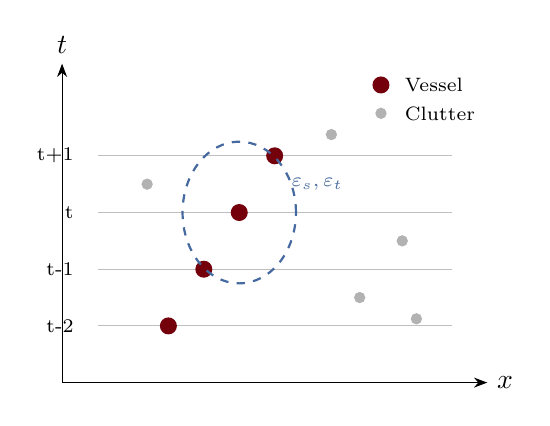
\begin{tikzpicture}[scale=0.9]
    % Axes
    \draw[-{Stealth}, black] (0,0) -- (6,0) node[right] {$x$};
    \draw[-{Stealth}, black] (0,0) -- (0,4.5) node[above] {$t$};
    
    % Time slices
    \foreach \y/\label in {0.8/t-2, 1.6/t-1, 2.4/t, 3.2/t+1} {
        \draw[gray!50] (0.5,\y) -- (5.5,\y);
        \node[left, font=\scriptsize] at (0.3,\y) {\label};
    }
    
    % Cluster points (boat trajectory) - garnet
    \foreach \x/\y in {1.5/0.8, 2.0/1.6, 2.5/2.4, 3.0/3.2} {
        \fill[garnet] (\x,\y) circle (0.12);
    }
    
    % Noise points - gray
    \foreach \x/\y in {4.2/1.2, 4.8/2.0, 3.8/3.5, 1.2/2.8, 5.0/0.9} {
        \fill[gray!60] (\x,\y) circle (0.08);
    }
    
    % Epsilon neighborhood (ellipse)
    \draw[slate, thick, dashed] (2.5,2.4) ellipse (0.8 and 1.0);
    \node[slate, font=\scriptsize] at (3.6,2.8) {$\varepsilon_s, \varepsilon_t$};
    
    % Legend
    \fill[garnet] (4.5,4.2) circle (0.12);
    \node[right, font=\scriptsize] at (4.7,4.2) {Vessel};
    \fill[gray!60] (4.5,3.8) circle (0.08);
    \node[right, font=\scriptsize] at (4.7,3.8) {Clutter};
\end{tikzpicture}
\end{document}
